\documentclass[12pt,a4paper,DIV=calc]{scrartcl}
\usepackage[protrusion=true,expansion=true]{microtype}

\usepackage{float}
\usepackage{amssymb}
\usepackage[utf8]{inputenc}
\usepackage[T1]{fontenc}
\usepackage{graphicx}
\usepackage[bookmarks=true,hidelinks=true,breaklinks=true]{hyperref}
\usepackage{mathptmx}
\usepackage{cleveref}
\usepackage{enumitem}
\usepackage[backend=biber,natbib=true]{biblatex}
\usepackage[scaled=.92]{helvet}
\bibliography{references.bib}


\begin{document}
\title{Seminar paper on Probabilistic Near-Duplicate Detection Using Simhash}
\author{Arne Beer, MN 6489196, University of Hamburg}
\date{08.07.2019}

\maketitle


\section{Introduction}

In the age of the modern Internet, many services depend in large parts on crawlers and proper document detection and duplication elimination, near duplicate document detection becomes a necessity.
Real time detection of which website has already been visited and whether a website is new or just has been edited are important tasks during crawling~\cite{paper:scaling_six_billion}.

Standard hashing functions are often inefficient and operate in $O(n^2)$ space requirements for RAM and computing time~\cite{book:hashing}.
At the same time, the size of available documents grow steadily.
Google's website index alone has multiple hundreds of billions of web pages and over 100 Petabyte in size, according to their information website~\cite{info:google_stats}.

This paper attends to the paper \emph{Seminar paper on Probabilistic Near-Duplicate Detection Using Simhash}~\cite{inproc:main}.
The main challenge tackled by this paper is to find all matching pairs of fingerprints withing a certain Hamming distance $h$.
At this time, the fasted implementation for this procedure has been \emph{Block-Permuted Hamming Search} (BPHS), which requires RAM space at least four times the size of the whole dataset.
The authors of~\cite{inproc:main} aim to design a new algorithm that allows significantly faster online and batch document comparison and furthermore reduces RAM requirements, in exchange for a small percentage of recall loss.

In the first chapters, the basics for understanding this topic will be explained.
Afterwards the proposed algorithm will be looked at and the authors' findings will be discussed.

\section{Conventional Hashing}

Hashing is a technique, which is used to map data of an arbitrary size to a fingerprint with some fixed size.
This procedure could be seen as a function  $f(i) \rightarrow j$, which produces a value $j$ from from any value $i$, where $j \in H$ and $H$ is the set of values of the fixed length $s$ with $s \in \mathbb{N}$.
Well-known hash functions are, for instance, \emph{MD5} or \emph{SHA265}.
These hashing functions are commonly used to check whether two files are absolutely identical or, for instance, to verify that a file has not been corrupted during transport.
This is possible, since these hashing functions are designed to flip half of the output hash bits on average, if an input bit changes~\cite{book:hashing}.
Without this property it would be easier to change the input without the hash signature being modified.
This would allow malicious third parties to, for instance, change code in a binary, without users being able to detect the change with the help of this hash and would require a full byte level comparison between the original and the copied file to verify its integrity.

If, on the other hand, one's goal is to find near duplicates, which are identical for the most part, but sometimes only differ by a few bits or bytes, this hashing approach immediately becomes useless, due to this property.
Due to the need for a hashing algorithm, that creates a fingerprint based on the features and structure of the input data, \emph{Simhash} has been created.


\section{Simhash}

\emph{Simhash} is a procedure used to create a fingerprint of a any kind of data.
This fingerprint can then be used to, for instance, inspect two files for similarity.

The process for creating such a fingerprint can completely differ depending on the features in the hashed data one is interested in.
In case one wants to find similar binary files, it would be reasonable to split the data into equal chunks and use these chunks as features.
For websites or documents, looking at the composition and structure of text could be a viable approach to select features for hashing
The original data can then be seen as a high dimensional vector of features.

The size of available features can vary significantly and is completely in the hand of the designer for each \emph{Simhash} implementation.
It's important to note, that there exists no clear guideline on which features of a data set are interesting and which features can be ignored.
The performance of a \emph{Simhash} implementation thereby also depends on the chosen features and the respective properties of the dataset.
Such features can be for instance binary chunks, file extension~\cite{inproc:simhash}, individual words, tags or URLs~\cite{inproc:main}.

\begin{figure}[H]
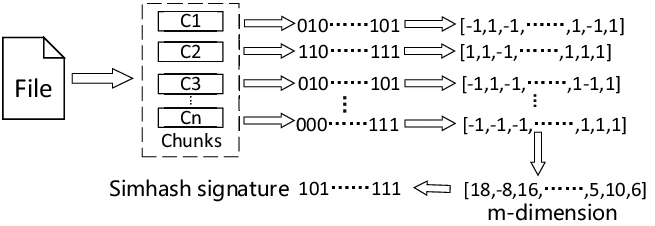
\includegraphics[scale=0.5]{./gfx/binary_chunk_fingerprint}
\centering
\caption{Process of calculating a \emph{Simhash} fingerprint.
A binary file split into chunks, which are then hashed.
Combined all hashes results in the desired fingerprint.~\cite{article:sampling-similarity}}\label{fig:gitalizer-relationship}
\end{figure}

After determining in which way feature are extracted from the original data, each feature is hashed and mapped onto a fingerprint, which represents the constellation of features.

The next challenge, which is the main topic this paper deals with, is to compare a fingerprint to all other fingerprints inside the given dataset.

\subsection{Weights and Hamming Distance}



\subsection{}



\subsection{Achievements of Session Juggler}


\section{Impact in the scientific community}


\section{Relevance as of 2018}


\printbibliography
\end{document}
